\chapter{Impedance estimation}
\label{chap:estimation}

The previous chapter showed how to design a multi-frequency experiment and digitally acquire the voltage and current signals fo the electrochemical cell, while this chapter discusses the methods used in this work to estimate instantanous impednace form the multi-frequency signals.
In Chapter \ref{ch:deis state art} I reported the three main methods for estimating impedance: STFT, DMFA and BLTVA. For its semplicity of implementation I used mainly the DMFA method and the STFT for the online computation of part of the impedance.
The novelty of this work is the use of the combination of DMFA and STFT to exploit the advantages of both: high frequency resolution of the DMFA for the low freuqncy band of the impedance spectrum and fast computation of the STFT for the high frequency band.
The STFT method was implemented online in the experiometn dataflow thanks to its modular design and multi-threaded excecution.

This chapter describes how impedance is estmiated off-line 
as used in the experiments presented later in the results part (Chapters \ref{chap:LTP}, \ref{chap:capacitor}, \ref{chap:anodes}), then I will described the signal workflow to estimate part of the impedance online with STFT method as it was used for the main result chapter on li-ion commercial batteries (Chapter \ref{chap:coins}).

\section{Off-line estimation with DMFA}
In this work I use the term \emph{off-line} to emphasize the difference with the \emph{on-line} approach that is descussed later in the chapter.
The off-line method is the traditional method used in system identification for which input and output mutlti-frequency signals are sampled for an integer number of periods and the instantanous frequency response funciton is estimated through a Fourier-transform-based analysis. 

In practice, the acuiredmulti-frequency data are stored in single files that contain either a whole electrochemical experiment (as for in Chapters \ref{chap:LTP}, \ref{chap:capacitor}, \ref{chap:anodes}) or the data of one technique of the entire sequence that deifned the experiment.
The latter is the case for long battery cycling (as in Chapter \ref{chap:coins}) so the estimation of the instantanous impednace for the whole experiment require to loop though single datasets and excute the DMFA algorithm for this.
In both cases, before starting the estimation algorithm the signal baseline was removed to reduce the Gibb's effect.
This procedure, referred as \emph{detrending}, is important in system identification to obtain clean Fourier spectra.
The linear detrending used here is the simplest of the detrending methods; better solution exist \cite{hallemansTrendRemovalMeasurements2022, lentkaMethodsTrendRemoval2019}, but they are computationally difficult for long signals like the ones in this work.

When excecuting the DMFA, the important parameters to choose are the filter function, its strength and its bandwidth.
Following the study of Chuckwu et. al \cite{chukwuStatisticalAnalysisMeasurement2022} as presented in Section \ref{sec:dmfa description}, in this work I used the symmteric Fermi-Dirac function as filter with a value $n$ of 8 that produces a flat band pass and fast roll-off.
The bandwidth, instead, varies by experiment since it is chosen as the inverse of the multisine period, corresponding to the maximum temporal resolution of the DMFA method.

\section{On-line processing and data reduction}
\label{On-line computation}

\subsection{Motivation}
Using the method of DMFA requires storing the complete signal of an experiment or a technique.
When the sample rate of the acquisition is high or the acquisition time is long, the ammount of disk-space occupied by the signals become significant.
The sample rate is determined by the maximum frequencies of the excitation wave (at least twice according to the Nyquist theorem) while the experiment time depend on the desired characterization of the system; charaterization of redox couple via cyclic voltammetry might last a few minutes while characterizing the intercalation in layered material takes hours, and the phenomena of battery aging appears in weeks.

Typically, batteries and other electrochemical systems responds to escitations from mHz up to few thausands of Hertz.
Sampling, for axample, the signals of as system at 500kHz creates 7.2\,GB per hour, filling up even the most spacious hard drives in a few days.
Employing dynamic impednace spectroscopy with high frequency excitations and for long time become unpractical under these circumstances, especially when interested in performing replicas or parallel cells measurments with the same computer.
Furthermore, integrating such measurment in more modest hardware, like micro-controllers, for the real time estimation of energy storage or generation devices is practically impossible.

\subsection{Strategy of the on-line processing}

This work provides a solution to the problem of data volume computing the high frequency band impedance on-line via STFT method over a short time window, then filtering and downsampling the windowed signal for the offline estimation of the lower band impedances via DMFA. 

The online processing of the multi-frequency signals is possible thanks to a software component excecuted inside the automation software described in previous chapter.
The online processing consist of the object \verb|PicoCalculator|, part of the \verb|DEIStools| module, which adds the possibilty of excecuting operations on the data streamed by the PicoScope device.
On its core, it simply adds in the streaming loop a condition that checks if the buffed data is long enough (i.e. the window of the STFT) to be processed.
The baseline of the signal is removed before excecuting the algorithm and no bell-shaped function is multiplied since it makes no difference for system drifting slowly as for the system studied in Chapter \ref{chap:coins}.
The workflow is schematically reported in Figure \ref{fig:DEIS automation workflow online}.

\begin{figure}
    \centering
    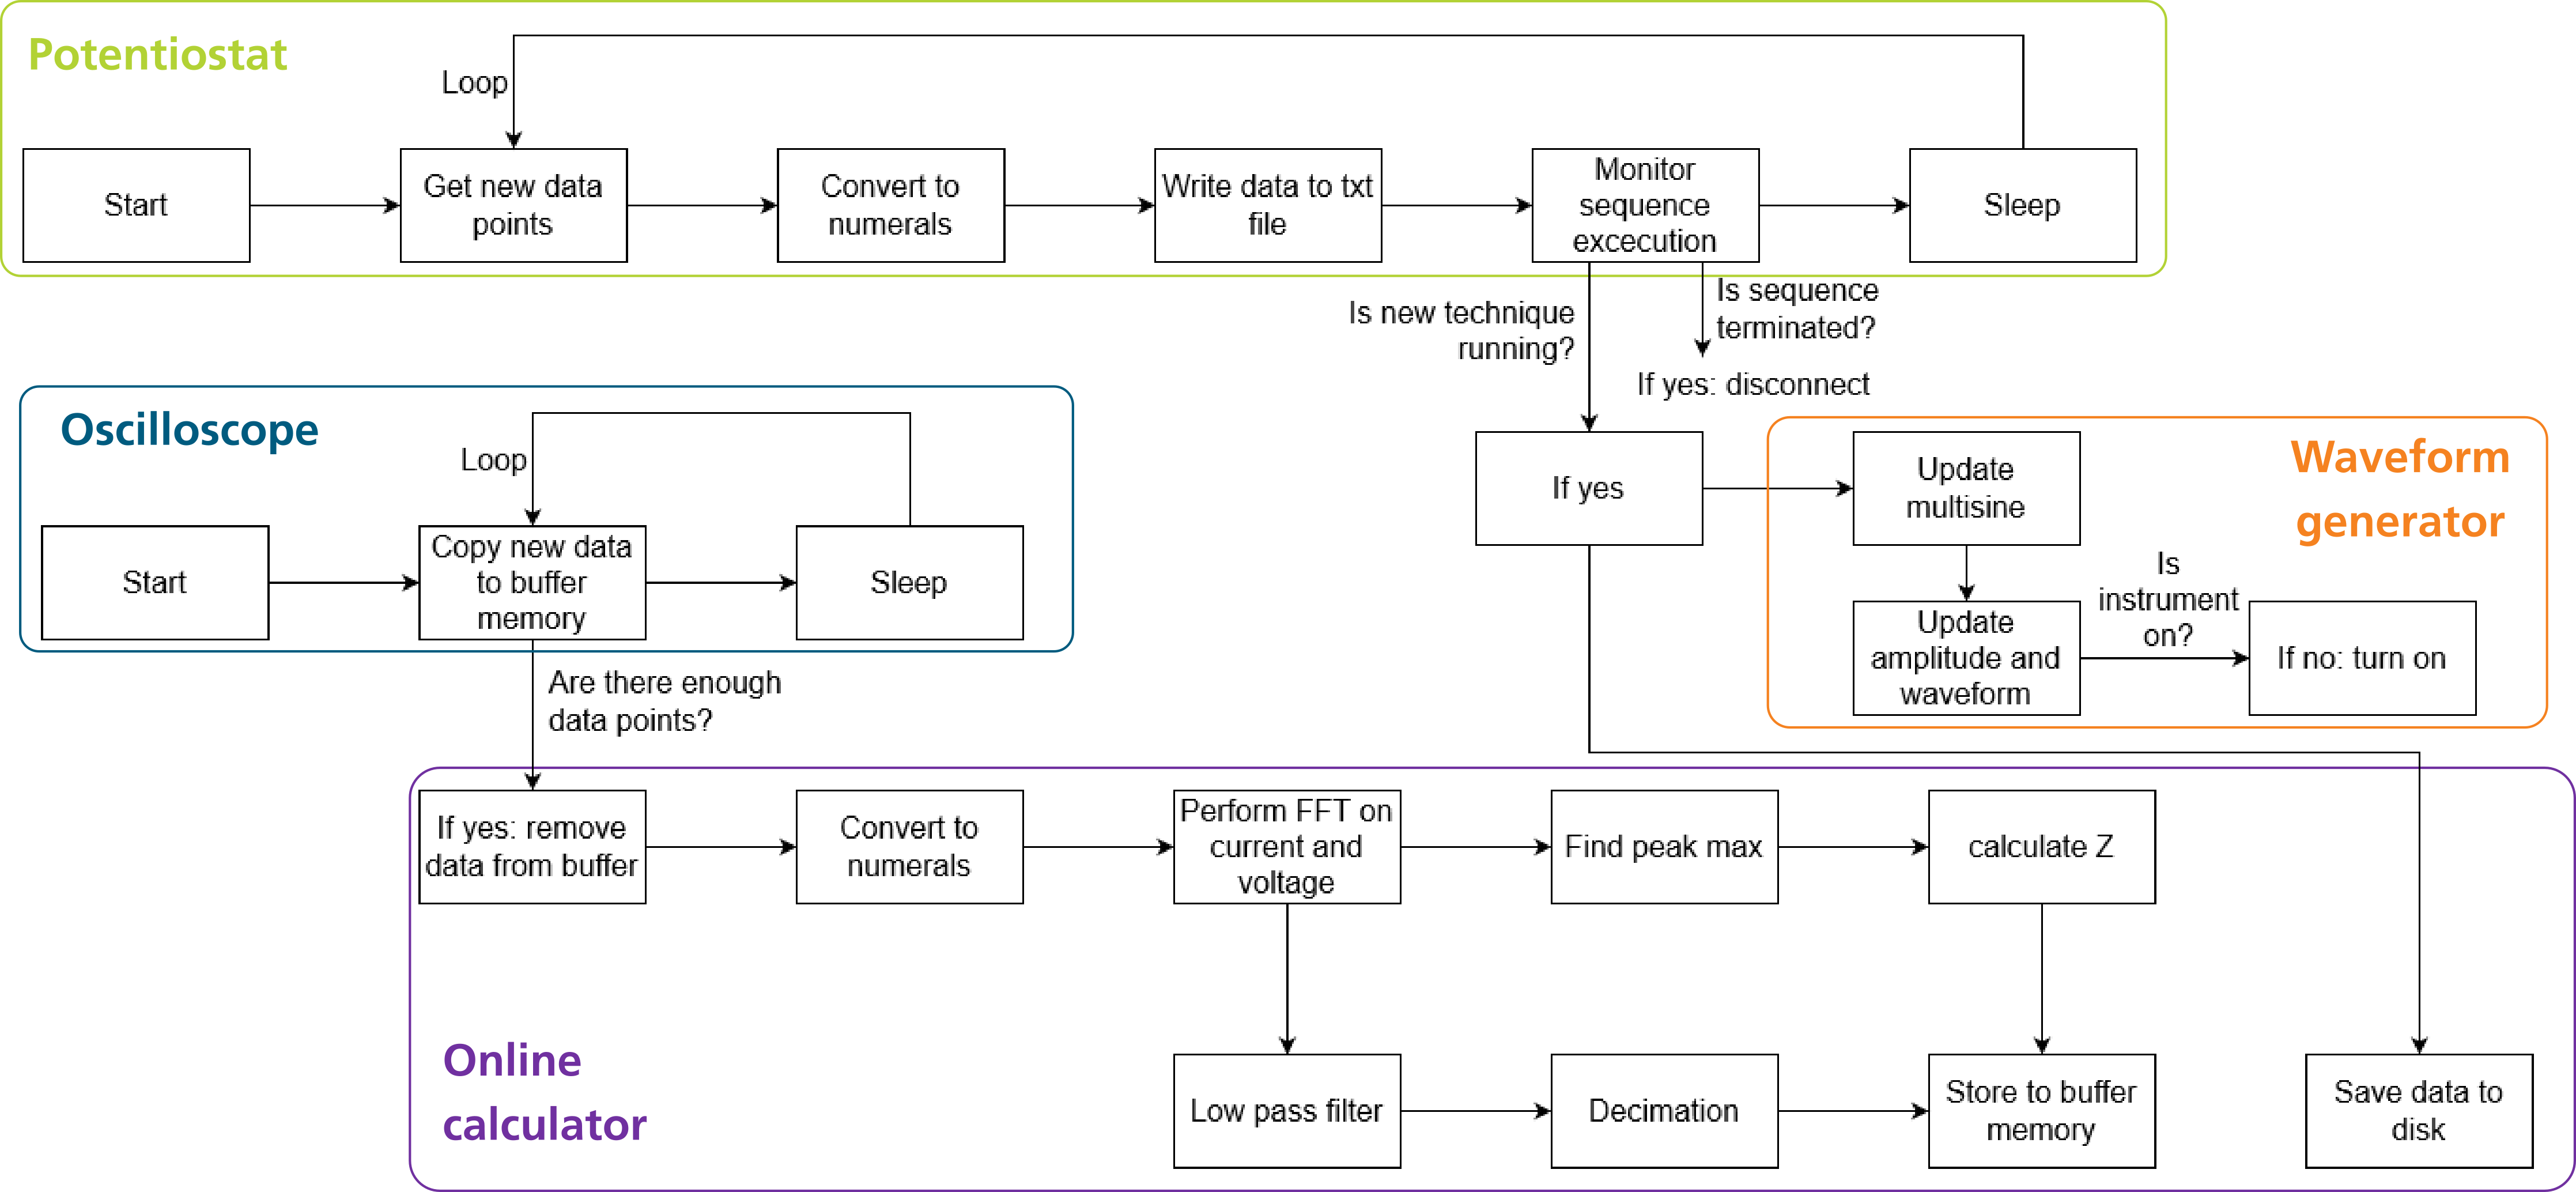
\includegraphics[width=\textwidth]{figures/acquisition/deis_workflow_online_calc.png}
    \caption{Schematics of the signal flow in an automated dynamic impedance spectroscopy experiment with online calculation of the high frequencies impedance.}
    \label{fig:DEIS automation workflow online}
\end{figure}

\subsection{Details of the data processing}

When a voltage and current blocks of data equivalent to the window length are acquired, \verb|PicoCalculator| copies the signals to another object, \verb|BlockCalculator|, that performs the following actions:
\begin{itemize}
    \item remove linear baseline of both signlas;
    \item perform the DFT of the signals;
    \item estimate the impedance of the high frequency band as ratio of the two fourier spectra at the frequencies of the excitation and store it;
    \item apply a Fermi-Diract function as low-pass filter;
    \item perform inverse DFT of the filtered signals;
    \item decimate the signals and store them.
\end{itemize}
The user must choose the low-pass filter critical frequency to remove all the frequency components estimated with the STFT method. 
The strategy is summarized in Figure \ref{fig:online processing scheme}.
\begin{figure}[H]
    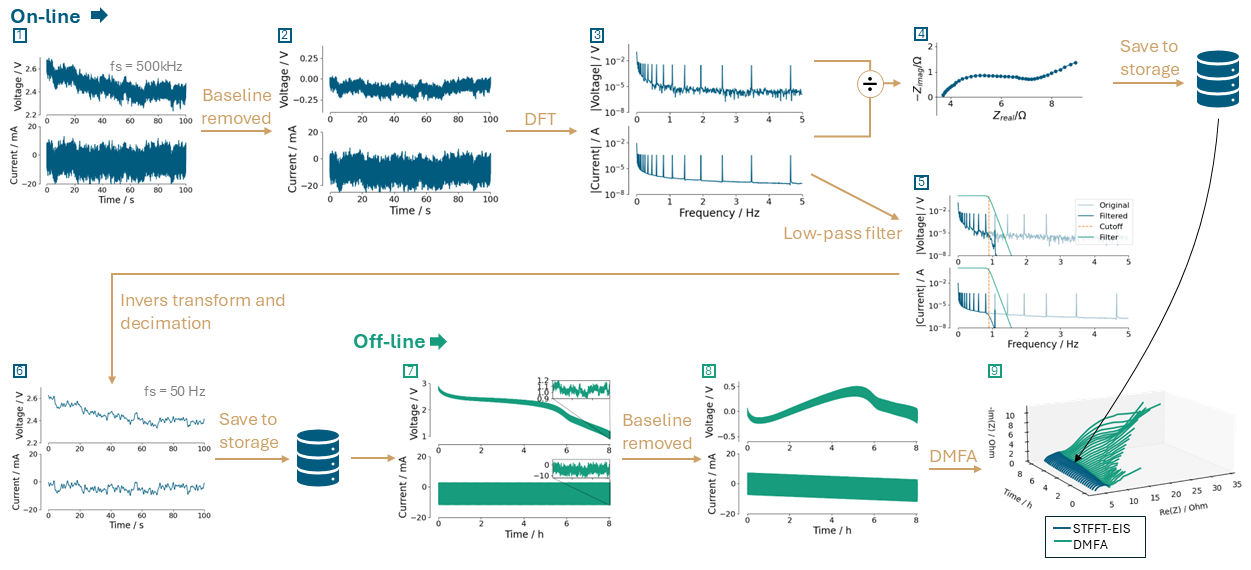
\includegraphics[width = \textwidth]{figures/estimation/computation_scheme.png}
    \caption{Schematics of the on-line processing.}
    \label{fig:online processing scheme}
\end{figure}

In this work I characterize with this combined method commercial lithium-ion batteries in the frequeny range 10mHz-200kHz. 
The online STFT was configured to compute the impedance of all the frequencies above 10Hz, so the low-pass filter choose a critical frequency was 8Hz.
For ease of implementation a performed the filtering by multiplying the 
The filter was the same symmetric Fermi-Dirac funtion used in the DMFA and was set with an $n$ value of 25 that produces a gain roll-off fast enough to bring the 10Hz signal to noise level. 
Later the DMFA is used to estimate impedance from 10mHz to 10Hz (exclueded) and the two are merged together to obtain the complete broadband impedance.
If the time resolution of the DMFA and the window length are the same there is no need to process the istantaneous impedances to match the time steps and the results of the two methods are simply concatenated.

In Appendix \ref{app:deis meas script} are reported examples on how to write scripts to configure the onlie computation of impednace and downsampling and integrate it in the automation software.

\subsection{Software limits}

Electrochemical methods applied to energy storage devices usually apply a drift between upper and lower limit of voltage (either in cyclic voltammetry or galvanostatic) or current (in potentiostatic).
When a multisine is applyed on top of the drift, it is important to know the average of the signals to accuratley compare it with the chosen limit instead of solely their latest value.
In this work I implemented an avarage signal calculator based on 
This avarage limit can be added to \verb|DEISChannel| (see Appendix \ref{app:deis meas script}) on the values working electrode voltage, cell voltage or current returned by the potentiostat.
When the object \verb|PicoCalculator| is used for the online computation of the impedance, the avarage of the signal can be estimated directly from the Fourier spectra of the windowed signals.

\subsection{Validation against DMFA}
Before implementing the STFT online in the acquisition dataflow, I simulated the process offline to very that the ouput of the STFT and downsampling procedure was not altering the impedance.
As example dataset I used the multi-frequency charging voltage and current obtained from a galvanostatic experiment at C/10 C-rate with a multisine in the range 10mHz-1kHz.
The cell used for the experiment is a lithium-ion coin cell of the same type used in the study prosented in Chapter \ref{chap:coins}.

Firstly, I verified that the downsampling and filtering was not causing any alteration of the frequency component, as reportedin figure \ref{fig:downsampling validation}.
As a low-pass filter I applied a Bessel filter - of order 7 and cut-off frequency 100 Hz - on data block of 100 s lenght.

\begin{figure}[H]
    \centering
    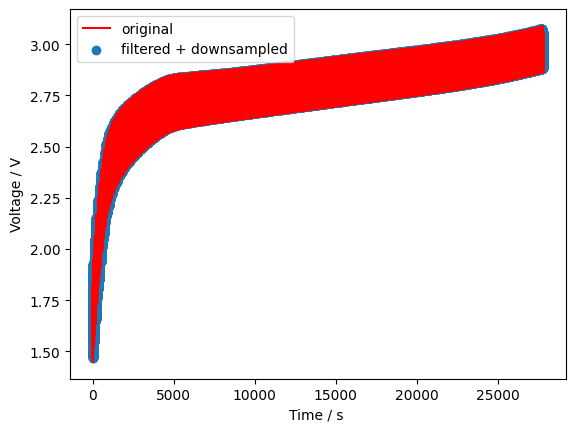
\includegraphics[width = 0.45\textwidth]{figures/estimation/orginal vs downsampled voltage charge.png}
    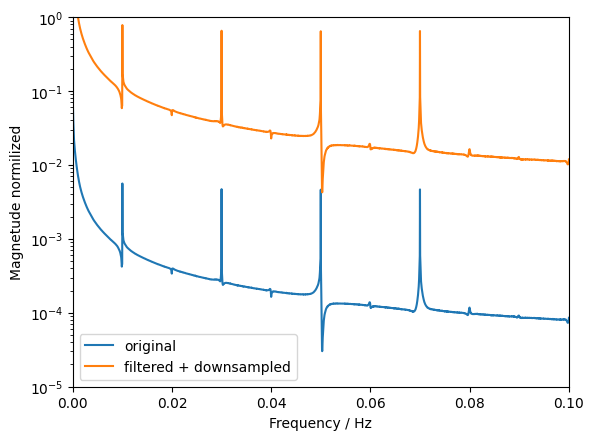
\includegraphics[width = 0.45\textwidth]{figures/estimation/orignal vs voltage DFT.png}
    \caption{Validation of frequincy content after downsampling.}
    \label{fig:downsampling validation}
\end{figure}

I estimated the impednace for all the frequencies in the multisine with the DMFA on the original dataset; then the impedance of high frequencies impedance on consecutive data windows with the STFT and estimated the low frequencies impedance on the downsample signals with the DMFA.
The coimparison in Figure \ref{fig: hybrid method validation} shows that no distortion is introduced by the low-pass filtering.

\begin{figure}[H]
    \centering
    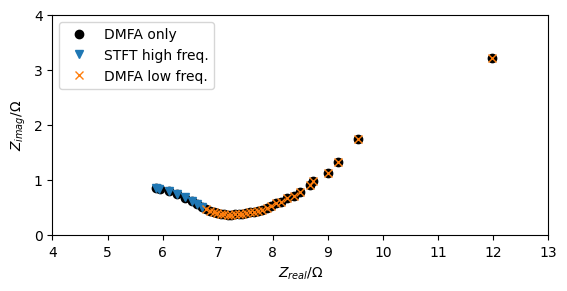
\includegraphics[width = \textwidth]{figures/estimation/mixed method validation.png}
    \caption{The use of a hybrid impedance esetimation method with STFT and DMFA gives the same result as using the DMFA for all the frequencies.}
    \label{fig: hybrid method validation}
\end{figure}

\section{Summary and limitations}
The use of a hybrid impedance estimation method allows for a real braod-band dynamic impedance spectroscopy to characterize the full spectrum of energy storage systems tyhat respond over multiple decades (7-8).
While the idea is valid, the practical implementation has some limitation due to the technical characteristic of the setup used.
Firstly, the ammount of calculations and memory managment could be optimized.
Now it is possible to run the algorithm on dedicated computer, but it is unlikley to work on micro-controllers.
Seocnd, the analyis in blocks of data using a multiplicative filter creates small discontinouties of circa 6mV between two consecutive signal blocks. 
While I could prove that the use of proper Finite Response Filter \footnote{This filter act on the time domain data by multiplication with the filter trasnfer function. This is the standard way of filtering in digital signal proccesing and can be easily implemented in micro-controller} with a Bessel filter returns undistorted data, for my limited software engneering skills I wasn't able to implement it in the software.
Nontheless the modularity of the automation software will permit to easly optimize each of the steps when needed.